\documentclass[preview]{standalone}
\usepackage{tkz-graph}
\begin{document}

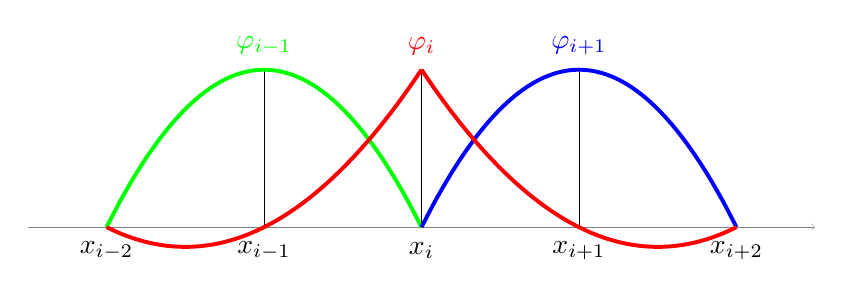
\begin{tikzpicture}
\draw[->,ultra  thin,color=gray] (0,0) -- (10, 0);
\draw[line width=0.1mm, color=black] (3,0) -- (3, 2);
\draw[line width=0.1mm, color=black] (5,0) -- (5, 2);
\draw[line width=0.1mm, color=black] (7,0) -- (7, 2);
\draw[green, line width = 0.5mm]   plot[smooth,domain=1:5] (\x, {2-0.5*(\x-3)^2});
\draw[blue, line width = 0.5mm]   plot[smooth,domain=5:9] (\x, {2-0.5*(\x-7)^2});
\draw[red, line width = 0.5mm]   plot[smooth,domain=1:5] (\x, {- 0.5*(\x-1) + 0.25*(\x-1)^2});
\draw[red, line width = 0.5mm]   plot[smooth,domain=5:9] (\x, {- 0.5*(\x-7) + 0.25*(\x-7)^2});
\draw (1, -0.3) node {$x_{i-2}$};
\draw (3, -0.3) node {$x_{i-1}$};
\draw (5, -0.3) node {$x_{i}$};
\draw (7, -0.3) node {$x_{i+1}$};
\draw (9, -0.3) node {$x_{i+2}$};
\draw[green] (3, 2.3) node {$\varphi_{i-1}$};
\draw[red] (5, 2.3) node {$\varphi_{i}$};
\draw[blue] (7, 2.3) node {$\varphi_{i+1}$};
\end{tikzpicture}

\end{document}



После: convert pdf to png
https://convertio.co/pdf-png/



 






